\documentclass{beamer}
\usetheme{Montpellier}
\usecolortheme{seahorse}

%\usepackage[slovak]{babel}
%\usepackage[utf8]{inputenc}

\usepackage{fontspec}
\usepackage{polyglossia}
\setdefaultlanguage{slovak}

\usepackage{pdfpcnotes}

\usepackage{tikz}
\usetikzlibrary{calc, fit}
\usetikzlibrary{patterns, shadings, shadows.blur}
\usetikzlibrary{decorations.pathmorphing,decorations.pathreplacing}
\usepgflibrary{decorations.markings}

% Modified from http://tex.stackexchange.com/a/17578/23342
% Center around any rect by redefining bounding box, can use node names
\tikzset{xcenter around/.style 2 args={execute at end picture={%
  \useasboundingbox let \p0 = (current bounding box.south west), \p1 = (current bounding box.north east),
                        \p2 = #1, \p3 = #2
                    in
        ({min(\x2 + \x3 - \x1,\x0)},\y0) rectangle ({max(\x3 + \x2 - \x0,\x1)},\y1);
}}}

\newcommand*{\FiguresPath}{figures}

\newcommand{\bigO}{\ensuremath{\mathcal{O}}}

\title{Cache-oblivious algoritmy a ich vizualizácia}
\author[Ladislav Pápay]{Ladislav Pápay \\ ~ \\ Vedúci: Mgr. Jakub Kováč, PhD.}
\date{}

\begin{document}

\frame{\titlepage}

\section{Úvod}
\begin{frame}
    \frametitle{Obsah práce}
    \begin{itemize}
        \item RAM model vs. cache-oblivious model
        \item Prehľad cache-oblivious algoritmov a DŠ
        \begin{itemize}
            \item Ich popis a analýza
        \end{itemize}
        \item Vizualizácia vybraných DŠ
    \end{itemize}
\end{frame}

\section{Pamäťový model}
\subsection{RAM model}
\begin{frame}
    \frametitle{RAM model}% ($\approx$ 1974, Hopcroft)}
    \emph{Random-Access Machine} -- stroj s náhodným prístupom k pamäti
    \begin{itemize}
        \item Klasický model pri časovej analýze algoritmov
        \item Prístup k ľubovolným dátam vyžaduje $\bigO(1)$ času
    \end{itemize}
\end{frame}

\subsection{Problémy RAM modelu}
\begin{frame}
    \begin{itemize}
        \item V skutočnosti však máme viac úrovní pamäte
        \item Rýchla pamäť je malá a drahá $\Rightarrow$ pamäťová hierarchia
    \end{itemize}
    \begin{center}
		\begin{tabular}{|l|l|l|}
			\hline
			Úroveň & Veľkosť & Odozva \\ \hline
			L1 & $\approx$ 128KiB & 4clk $\approx$ 1ns (pri 3.5GHz) \\ \hline
			L2 & $\approx$ 1MiB & 10-12clk $\approx$ 3ns (pri 3.5GHz) \\ \hline
			L3 & $\approx$ 8MiB & 20-50clk $\approx$ 10ns (pri 3.5GHz) \\ \hline
			RAM & $\approx$ 4GiB & $\approx$ 100ns \\ \hline
			Disk & $\approx$ 1TiB & $\approx$ 0.1-10ms \\
			\hline
		\end{tabular}
	\end{center}
	\begin{itemize}
	    \item Rozdiel v čase môže byť až 10\,000\,000-násobný
	    \item Môžeme dosiahnuť lepšiu rýchlosť algoritmu ak rozlišujeme ``pomalé'' a ``rýchle'' prístupy
	\end{itemize}
\end{frame}

\subsection{External-memory model}
\begin{frame}
    \frametitle{External-memory model}% (1988, Aggarwal, Vitter et al.)}
	\begin{columns}[T]
		\begin{column}{.4\textwidth}
			\begin{itemize}
				\item Cache celkovej veľkosti $M$
				\item Obsahuje $\frac{M}{B}$ blokov veľkosti $B$
				\item Disk neobmedzenej veľkosti, tiež zložený z blokov
			\end{itemize}
		\end{column}
		\begin{column}{.6\textwidth}\raggedleft
		    \resizebox{\textwidth}{!}{%
                
\begin{tikzpicture}

\newcommand{\width}{4}
\newcommand{\height}{1}
\newcommand{\cacheheight}{8}
\newcommand{\cachebox}{\height}
\newcommand{\cachewidth}{4} % TODO divide?
\newcommand{\off}{1}
\newcommand{\diskoff}{3*\width}

\newcommand{\jaggedsep}{0.25}

\newcommand{\arrangle}{20}
\newcommand{\arroff}{1}

\foreach \i in {1,...,\cacheheight}
{
\draw [thick] (0, \i*\height-\height) rectangle (\width, \i*\height);
}

\foreach \i in {1,...,\cachewidth}
{
\draw [thick] (\i*\cachebox-\cachebox, 0) rectangle (\i*\cachebox, \height);
}

\draw [thick, |-|] (0,-\off) -- (\width, -\off) node [midway, fill=white,minimum width=2cm] {\Huge $B$};
\draw [thick, |-|] (-\off,0) -- ++ ($(0, \cacheheight*\height) $) node [midway, fill=white, minimum height=2cm] {\Huge $\frac{M}{B}$};

% Dont draw bottom edge
\foreach \i in {2,...,\cacheheight}
{
\draw [thick](\diskoff, \i*\height-\height) rectangle (\diskoff+\width, \i*\height);
}
\draw [thick] (\diskoff, 0) -- (\diskoff, \height);
\draw [thick] (\diskoff+\width, 0) -- (\diskoff+\width, \height);
%\raggedline{(\diskoff, 0) -- (\diskoff+\width, 0)}
\draw [thick] ($(\diskoff-0.5, -0.5)$) -- ++(1, 1) -- ++(1, -1) -- ++(1, 1) -- ++(1, -1) -- ($(\diskoff+\width+0.5, 0.5)$);
\draw [thick] ($(\diskoff-0.5, -0.5-\jaggedsep)$) -- ++(1, 1) -- ++(1, -1) -- ++(1, 1) -- ++(1, -1) -- ($(\diskoff+\width+0.5, 0.5-\jaggedsep)$);

\draw [thick, |-] (\diskoff+\width+\off,\cacheheight*\height) -- ++ ($(0, -\cacheheight*\height+\height) $) node [midway, fill=white, minimum height=1cm] {\Huge $\infty$} node [pos=1, fill=white] {\Huge $\vdots$};

\coordinate (BBL) at (0.5*\diskoff, 0.5*\height*\cacheheight);
\coordinate (BTR) at ($ (BBL) +(\width, \height) $);
\coordinate (BC) at ($ 0.5*(BBL) + 0.5*(BTR) $);
\draw [thick] (BBL) rectangle (BTR);

\node at (0.5*\width, \height*\cacheheight+\off) {\Huge Cache};
\node at (0.5*\width+\diskoff, \height*\cacheheight+\off) {\Huge Disk};
%\node at ($ (BC) + (0, 0.5*\height+\off) $) {\Huge Presúvaný blok};
\node at (BC) {\Large Presúvaný blok};

\coordinate (LB) at (\width, 0.5*\height*\cacheheight);
\coordinate (RB) at ($ (LB) + (\diskoff-\width, 0) $);
\coordinate (LT) at ($ (LB) + (0, \height) $);
\coordinate (RT) at ($ (RB) + (0, \height) $);

%\draw [->,thick,decoration={markings,mark=at position 1 with {\arrow[scale=2]{>}}},postaction={decorate}]  ($(LB) + (-\arrangle:\arroff) $) to  [out=-\arrangle,in=180+\arrangle] ($(RB) + (180+\arrangle:\arroff) $);
%\draw [->,thick,decoration={markings,mark=at position 1 with {\arrow[scale=2]{>}}},postaction={decorate}]  ($(RT) + (180-\arrangle:\arroff) $) to  [out=180-\arrangle,in=\arrangle] ($(LT) + (\arrangle:\arroff) $);

\draw [->,ultra thick,]  ($(LB) + (-\arrangle:\arroff) $) to  [out=-\arrangle,in=180+\arrangle] node[below,midway]{\huge Zápis} ($(RB) + (180+\arrangle:\arroff) $);
\draw [->,ultra thick]  ($(RT) + (180-\arrangle:\arroff) $) to  [out=180-\arrangle,in=\arrangle] node[above,midway]{\huge Čítanie} ($(LT) + (\arrangle:\arroff) $);


\end{tikzpicture}    
            }    
		\end{column}
	\end{columns}
	\bigskip
	Môžeme pracovať len s dátami v cache.
	
    Počíta sa počet prenesených blokov (operácie v cache sú zadarmo).
    
	
	%\input{../figures/external_memory_inkscape/drawing.eps_tex} 
\end{frame}

\begin{frame}
	\frametitle{External-memory model}
	\begin{itemize}
		\item Známe tiež ako cache-aware (kontrast voči cache-oblivious)
		\item Poznáme $B$ a $M$, každá operácia čítania/zápisu na disk je (potenciálne) explicitne vykonaná algoritmom
	\end{itemize}
    Problémy cache-aware algoritmov:
    \begin{itemize}
    		%\item Ak je cache plná, musí vybrať, ktorý blok zahodí (a jeho obsah treba zapísať na disk)
            \item Čo ak sa zmenia parametre $B$ alebo $M$?
		    \item Čo v prípade viac úrovní? Treba pre každú susediacu dvojicu poznať $B, M$  a spravovať bloky
    \end{itemize}
	\pnote{Pri zahadzovani bloku v cache ak bol zmeneny treba zapisat}
	\pnote{B pre disk/ram je cca 4KB}
	\pnote{Zistenie B a M - pri kompilacii, za behu?}
	\pnote{Treba pri zmene prekompilovat? Prepisat algoritmus}
	\pnote{L3 - RAM : 10x pomalsie, 100x vacsie}
	\pnote{RAM - Disk: 1 000x - 100 000x pomalsie, 1000x vacsie}
\end{frame}

\subsection{Cache-oblivious model}
\begin{frame}
	\frametitle{Cache-oblivious model}% (1999, Prokop, Frigo et al.)}
	\begin{itemize}
		\item Chceme (asymptoticky) rovnaký počet presunov ako optimálny cache-aware algoritmus, ale bez znalosti parametrov $B$ a $M$
		\begin{itemize}
		    \item Tieto parametre používame počas analýzy, ale algoritmus nepozná a nie je navrhnutý pre žiadne konkrétne hodnoty
		\end{itemize}
		\item Rovnaká architektúra, presun blokov prebieha automaticky
		\begin{itemize}
			\item Predpokladá optimálne nahrádzanie blokov (offline), ale FIFO/LRU je len konštantne horšie
		\end{itemize}
	\end{itemize}
	Výhody tohto prístupu:
	\begin{itemize}
	    \item Funguje pri zmene parametrov bez úprav
	    \item Funguje pre všetky susedné dvojice v pamäťovej hierarchii
	\end{itemize}
	\pnote{Pozname pri analyze, ale nie pocas behu}
\end{frame}


\newcommand{\amort}{{\small \textit{amort.}}}
\newcommand{\toprule}{\hline}
\newcommand{\bottomrule}{\hline}
\newcommand{\aware}{Cache-aware}
\newcommand{\obliv}{Cache-oblivious}

\section{Algoritmy a dátové štruktúry}
\begin{frame}
    \includegraphics[width=\textwidth]{table}
\end{frame}

\begin{frame}
    \includegraphics[width=\textwidth]{table_color}
\end{frame}


\begin{frame}
    \frametitle{Vyhľadávacie stromy}
    \begin{itemize}
        \item Často používaná dátová štruktúra
        \begin{itemize}
            \item Napríklad databázové systémy, kde máme veľa dát -- oplatí sa optimalizovať pamäťové presuny
        \end{itemize}
        \item Cache-aware riešenie -- B-stromy s vetvením $\bigO(B)$
        \begin{itemize}
            \item Všetky operácie vykonajú $\bigO(\log_B N)$ pamäťových presunov
            \item Optimálne riešenie, ale potrebuje poznať $B$
        \end{itemize}
        \item Existujú porovnateľné cache-oblivious riešenia
        \item Najskôr sa pozrime na statický vyhľadávací strom
        \begin{itemize}
            \item Na začiatku vybudujeme
            \item Potom už len vyhľadávanie, bez zmien
        \end{itemize}
    \end{itemize}
\end{frame}

\subsection{Statický strom}
\begin{frame}
    \frametitle{Statický strom v BFS usporiadaní}
    \begin{itemize}
        \item Jednoduchý spôsob ako uložiť binárny strom v pamäti -- pole, pričom synovia vrcholu $A[x]$ sú $A[2x]$ a $A[2x+1]$
    \end{itemize}

    \centerline{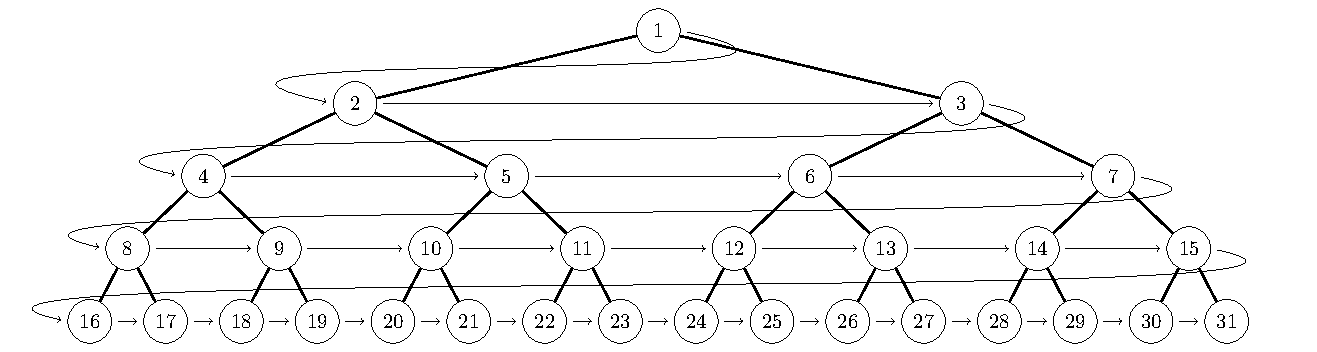
\includegraphics[width=1.1\textwidth]{../figures/vEB_tree/node_order_naive}}
    \begin{itemize}
        \item Vyhľadávanie ale vykoná aspoň $\Omega(\log\frac{N}{B})$ presunov
        \begin{itemize}
            \item Horšie ako cache-aware B-stromy
            \item V rovnakom bloku sa totiž načítajú prevažne zbytočné vrcholy
        \end{itemize}
    \end{itemize}
\end{frame}

\begin{frame}
    \frametitle{Statický strom vo vEB usporiadaní}
    \begin{itemize}
        \item \emph{van Emde Boasovo} usporiadanie (podľa vEB stromov)
        \begin{itemize}
            \item Rozdelíme uprostred na horný podstrom a $\sqrt{N}$ spodných podstromov veľkosti $\sqrt{N}$
            \item Tie rekurzívne rozdelíme a uložíme do súvislého bloku pamäte
        \end{itemize}
    \end{itemize}
    \resizebox{\textwidth}{!}{%
        \begin{tikzpicture}

% Triangle
\newcommand{\width}{8}
\newcommand{\height}{4}
\newcommand{\hoff}{0.25}
\newcommand{\voff}{0.25}
% Memory layout box
\newcommand{\memoff}{0.5}
\newcommand{\memw}{1}
\newcommand{\memh}{1}


\newcommand{\trianglecenter}[4]{
  \coordinate (#1) at ($1/3*(#2)+1/3*(#3)+1/3*(#4)$);
}

% Big Left/Right/Top
\coordinate (BL) at (0, 0);
\coordinate (BR) at (\width, 0);
\coordinate (BT) at (\width/2, \height);
% Top Left/Right/Top
\coordinate (TL) at (0.25*\width + \hoff, 0.5*\height);
\coordinate (TR) at (0.75*\width - \hoff, 0.5*\height);
\coordinate (TT) at ($ (BT)+(0, -\voff) $);
% Left Left/Right Right
\coordinate (LL) at ($ (\voff, \voff) + (\hoff, 0) $);
\coordinate (RL) at ($ (\width - \voff, \voff) - (\hoff, 0) $);
% Left+Right Center
\coordinate (LRC) at (0.5*\width, \voff);
\coordinate (LR) at ($ (LRC) - (0.5*\hoff, 0) $);
\coordinate (RR) at ($ (LRC) + (0.5*\hoff, 0) $);
% Centers
\trianglecenter{BC}{BL}{BR}{BT}
\trianglecenter{TC}{TL}{TR}{TT}
\trianglecenter{LC}{LL}{LR}{TL}
\trianglecenter{RC}{RL}{RR}{TR}

% Outer triangle
\draw [thick] (BL) -- (BR) -- (BT) -- (BL);
% Inner triangles
\draw (TL) -- (TR) -- (TT) -- (TL);
\draw (LL) -- (TL) -- (LR) -- (LL);
\draw (RL) -- (TR) -- (RR) -- (RL);

\node at (BC) {\Huge $\cdots$};
\node at (TC) {\Huge $\tau_0$};
\node at (LC) {\Huge $\tau_1$};
\node at (RC) {\Huge $\tau_k$};

% Layout in memory
\coordinate (M0LT) at ($ (BL) - (0, \memoff) $);
\coordinate (M0RB) at ($ (M0LT) + (\memw, -\memh) $);
\coordinate (M1RT) at ($ (M0RB) + (\memw, \memh) $);
\coordinate (M3RT) at ($ (BR) - (0, \memoff) $);
\coordinate (M3LB) at ($ (M3RT) - (\memw, \memh) $);

\draw (M0LT) rectangle (M0RB);
\draw (M0RB) rectangle (M1RT);
\draw (M1RT) rectangle (M3LB);
\draw (M3LB) rectangle (M3RT);

\node at ($ (M0LT)!0.5!(M0RB) $) {\huge $\tau_0$};
\node at ($ (M0RB)!0.5!(M1RT) $) {\huge $\tau_1$};
\node at ($ (M1RT)!0.5!(M3LB) $) {\huge $\dots$};
\node at ($ (M3LB)!0.5!(M3RT) $) {\huge $\tau_k$};


\end{tikzpicture}    
    }  
    \begin{itemize}
        \item V rovnakom bloku sa nachádza časť relevantného podstromu presunov
        \item Vyhľadávanie vykoná $\bigO(\log_B N)$
    \end{itemize}
\end{frame}

\begin{frame}
    \frametitle{Ukážka stromu vo vEB usporiadaní}
    \centerline{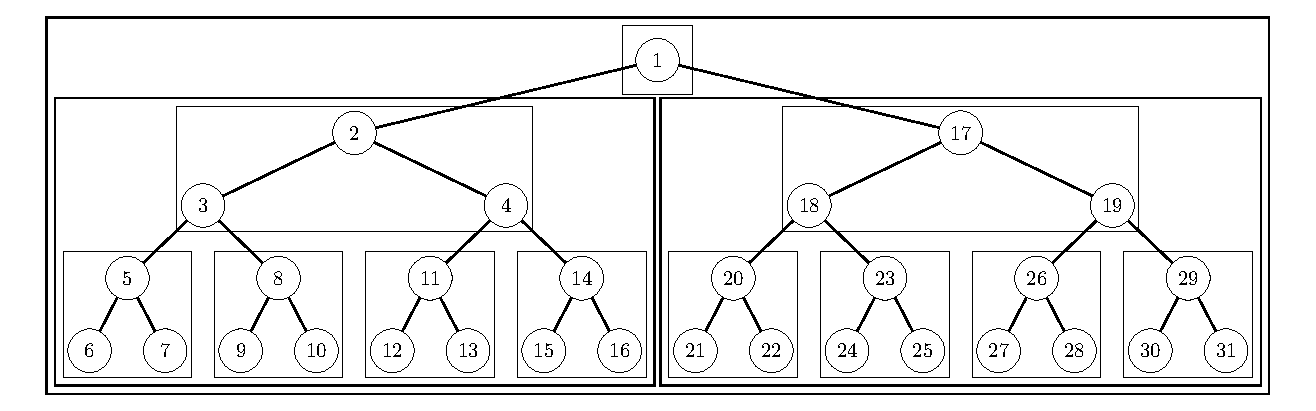
\includegraphics[width=1.1\textwidth]{../figures/vEB_tree/node_order_veb}}
\end{frame}

\begin{frame}
    \frametitle{Ďalšie štruktúry}
    \begin{itemize}
        \item Usporiadané pole
        \begin{itemize}
            \item Udržiava usporiadanú postupnosť prvkov v súvislom poli
            \item Umožňuje efektívne vkladať na ľubovolné miesto
        \end{itemize}                

        \item Dynamický vyhľadávací strom
        \begin{itemize}
            \item Kombinácia statického vEB stromu a usporiadaného poľa
            \item Podobné výsledky ako cache-aware B-stromy
        \end{itemize}        
    \end{itemize}
\end{frame}

\begin{frame}
    \frametitle{Porovnanie počtu pamäťových presunov}
    {\renewcommand{\arraystretch}{1.5}
    \begin{tabular}{lll}
        \hline \multicolumn{3}{c}{\textbf{Cache-aware B-strom}} \\ \hline
        Vyhľadávanie & Vkladanie & Prechod \\ \hline
        $\bigO(\log_B{N})$ & $\bigO(\log_B{N})$ & $\bigO(\frac{K}{B})$ \\
        \\
        \hline \multicolumn{3}{c}{\textbf{Cache-oblivious dynamický strom}} \\ \hline 
        Vyhľadávanie & Vkladanie & Prechod \\ \hline
        $\bigO(\log_B{N})$ & $\bigO(\log_B{N}+\frac{\log^2{N}}{B})$ \amort & $\bigO(\frac{K}{B})$  \\
        $\bigO(\log_B{N})$ & $\bigO(\log_B{N})$ \amort & $\bigO(\frac{K}{\min\{B,\log N\}})$
    \end{tabular}
    }
    \pnote{Prechod = SCAN}
\end{frame}

\section{Vizualizácie}
\begin{frame}
    \frametitle{Vizualizácie}
    \begin{itemize}
        \item Pridanie týchto dátových štruktúr do \emph{Gnarley Trees} (alg-vis)
        \item Krokovanie s animáciami, undo/redo
        \item Vysvetlenie krokov (v angličtine a slovenčine)
        \item Simulácia cache, nastaviteľné parametre $B$ a $M$
    \end{itemize}
    \begin{center}
        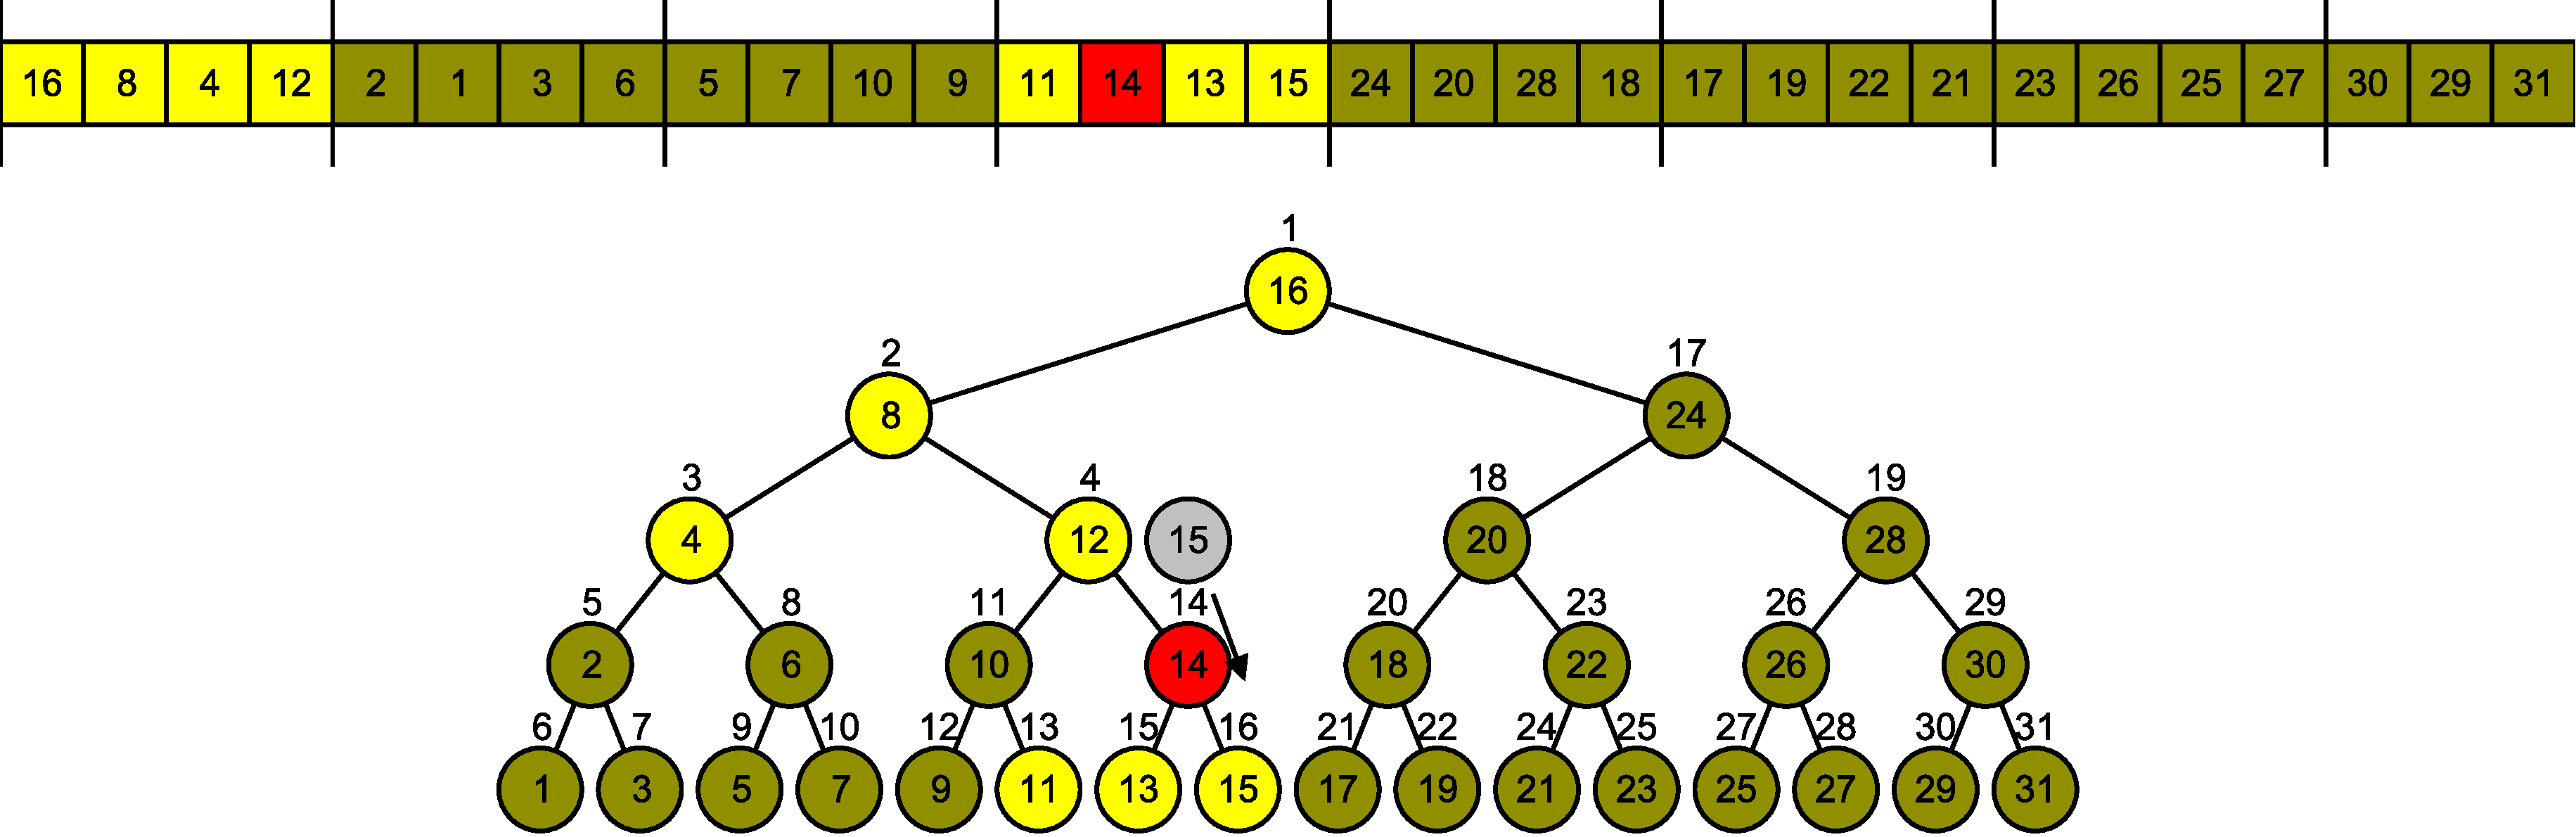
\includegraphics[width=\textwidth]{../figures/screenshots/cachesim_big_step4}
    \end{center}
    \pnote{alg-vis (Gnarley trees) - Jakub Kovac, 2007}
\end{frame}

\begin{frame}[plain]
\begin{center}
{\Large Ukážka vizualizácií \dots}
\end{center}
\end{frame}

\section{Algoritmy a dátové štruktúry}
\subsection{Statický vyhľadávací strom vo vEB usporiadaní}
\begin{frame}
    \frametitle{Analýza}
    \begin{itemize}
        \item Vyhľadávanie ako v klasickom BST (cache-ignorant prístup)
        \begin{itemize}
            \item Pozrime sa na takú úroveň delenia, že sú podstromy $\le B$ a teda zmestia sa do najviac dvoch blokov
            \item Tieto podstromy majú výšku $< \lg{B}$ ale $\ge \frac{1}{2}\lg{B}$
            \item Vyhladávanie prejde cestu od koreňa do listu dĺžky $\lg N$
            \item Prejdeme najviac cez $\frac{\lg N}{\frac{1}{2}\lg{B}}$ podstromov a na každý treba najviac 2 pamäťové presuny
        \end{itemize}
        \item Spolu teda $\bigO(\log_{B}{N})$ čo je spodná hranica pre external-memory model
    \end{itemize}
    \pnote{Analogia v cache-aware je B-strom}
\end{frame}

\subsection{Ordered file}
\begin{frame}
    \frametitle{Ordered file}
    \begin{itemize}
        \item Problém: udržiavať usporiadanú postupnosť prvkov, možnosť vkladať/odstraňovať, ako pole veľkosti $\bigO(N)$ $\Rightarrow$ medzery $O(1)$, vieme rýchlo prechádzať
        \item Riešenie: rozdelíme súvislé pole na imaginárne bloky veľkosti $\bigO(\log N)$ a vyrobíme nad nimi imaginárny úplný binárny strom
        \item {\em Hustota} vrcholu bude $\frac{\text{počet plných}}{\text{kapacita}}$, udržiavame podla istých hraníc aby nebolo príliš plné (nie je kam vložiť) ani príliš prázdne (pomalé prechádzanie)
    \end{itemize}
    \pnote{Hranice hustoty:}
    \pnote{Listy: 1/4 - 1}
    \pnote{Koren: 1/2 - 3/4}
\end{frame}

\begin{frame}
\begin{center}
        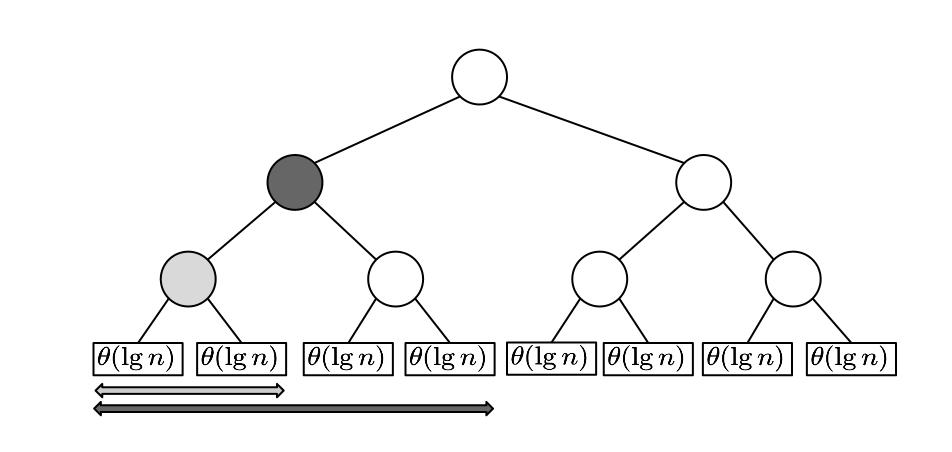
\includegraphics[width=0.8\textwidth,]{../figures/downloaded_dont_use/fig2-ofm.jpg}
    \end{center}
\end{frame}

\begin{frame}
    \frametitle{Operácie}
    \begin{itemize}
        \item {\em Vloženie prvku}: Upravíme blok a postupujeme hore v strome, kým nenájdeme vrchol, ktorý má hustotu v medziach a rovnomerne prerozdelíme prvky v príslušných blokoch
        \item {\em Zmazanie prvku} podobne
        \item Každá operácia upraví súvislý interval veľkosti $\bigO(\lg^2 N)$
    \end{itemize}
    \pnote{Imaginarny strom, scan v dvoch smeroch}
    \pnote{Odhad - amortizovane, dá sa aj worst-case}
    \pnote{Conjencture lowerbound}    
\end{frame}

\subsection{Dynamický strom}
\begin{frame}
    \frametitle{Dynamický strom}
    \begin{itemize}
        \item Skombinujeme predošlé dve štruktúry a dostaneme dynamický vyhľadávací strom
        \item Máme OF v ktorom sú kľúče a medzery, použijeme ako listy pre BST uložený v vEB layoute
        \item Vo vnútorných uzloch ukladáme maximum z podstromov
    \end{itemize}
    \begin{center}
        %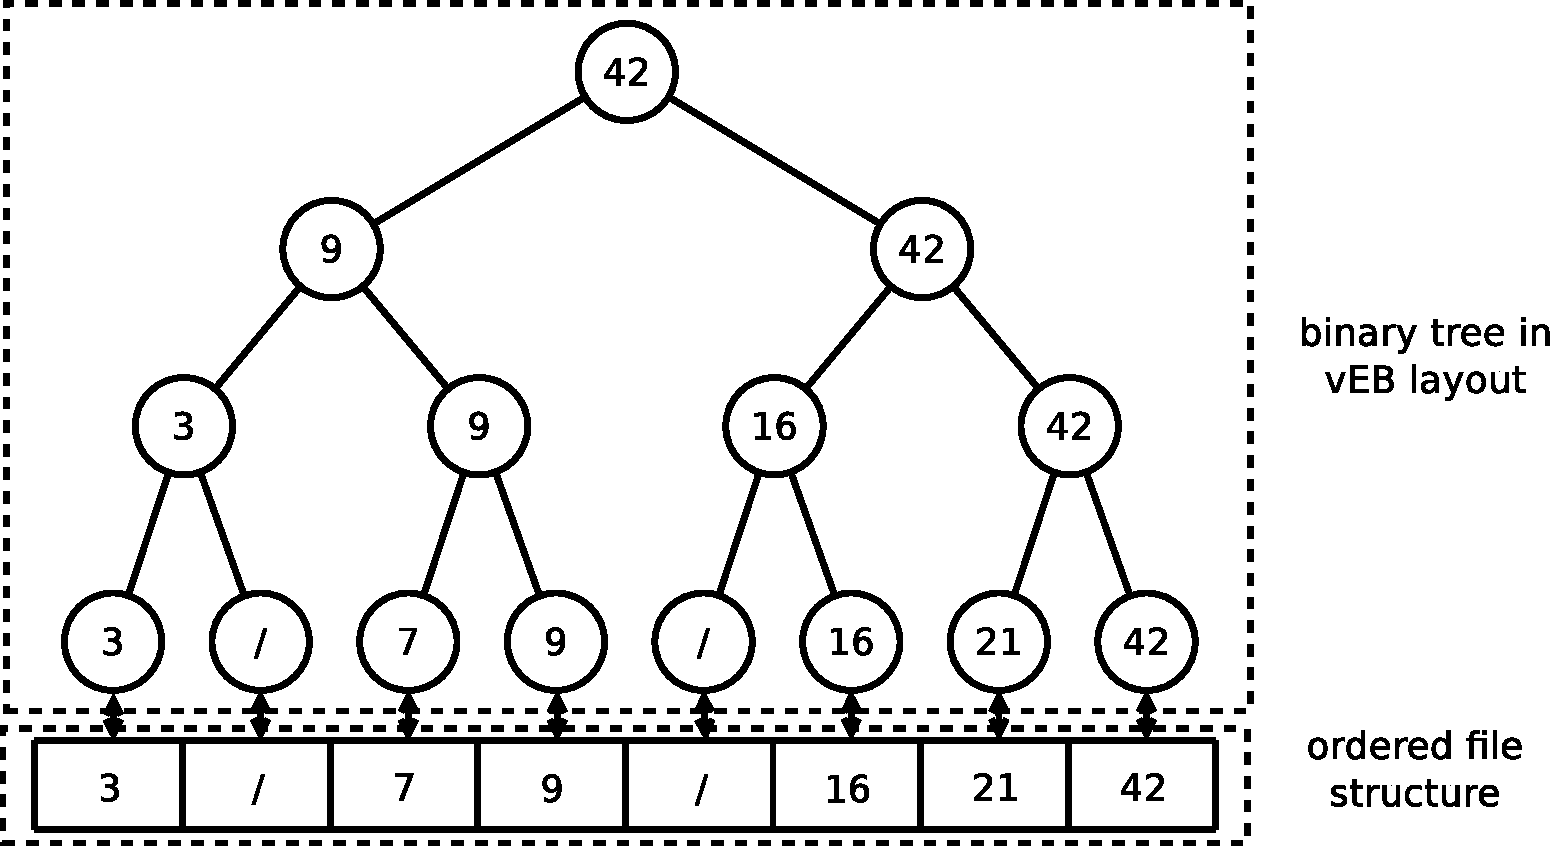
\includegraphics[height=0.5\textheight]{../figures/downloaded_dont_use/vEBpOFM.pdf}
        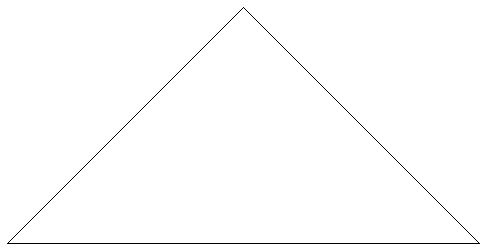
\includegraphics[height=0.5\textheight]{../figures/dynamic_tree/overview}
    \end{center}
\end{frame}

\begin{frame}
    \begin{itemize}
        \item Vyhľadávanie: rovnako ako v statickom $\bigO(\log_B N)$
        \item Vkladanie
        \begin{itemize}
            \item Nájdeme nasledujúci kľúč v OF, vložíme nový pred neho
            \item Musíme upraviť strom pre zmenený interval veľkosti $\bigO(\lg^2 N)$
            \item Prechod cez zasiahnuté vnútorné uzly vyžaduje $\bigO(\frac{\lg^2 N}{B})$ pamäťových operácií
        \end{itemize}
        \item Vkladanie a odstraňovanie spolu potrebuje $\bigO(\log_B N + \frac{\lg^2 N}{B})$
        \item Dá sa zredukovať na $\bigO(\log_B N)$ ak ukladáme $\bigO(\log N)$ bloky
    \end{itemize}
    \begin{center}
        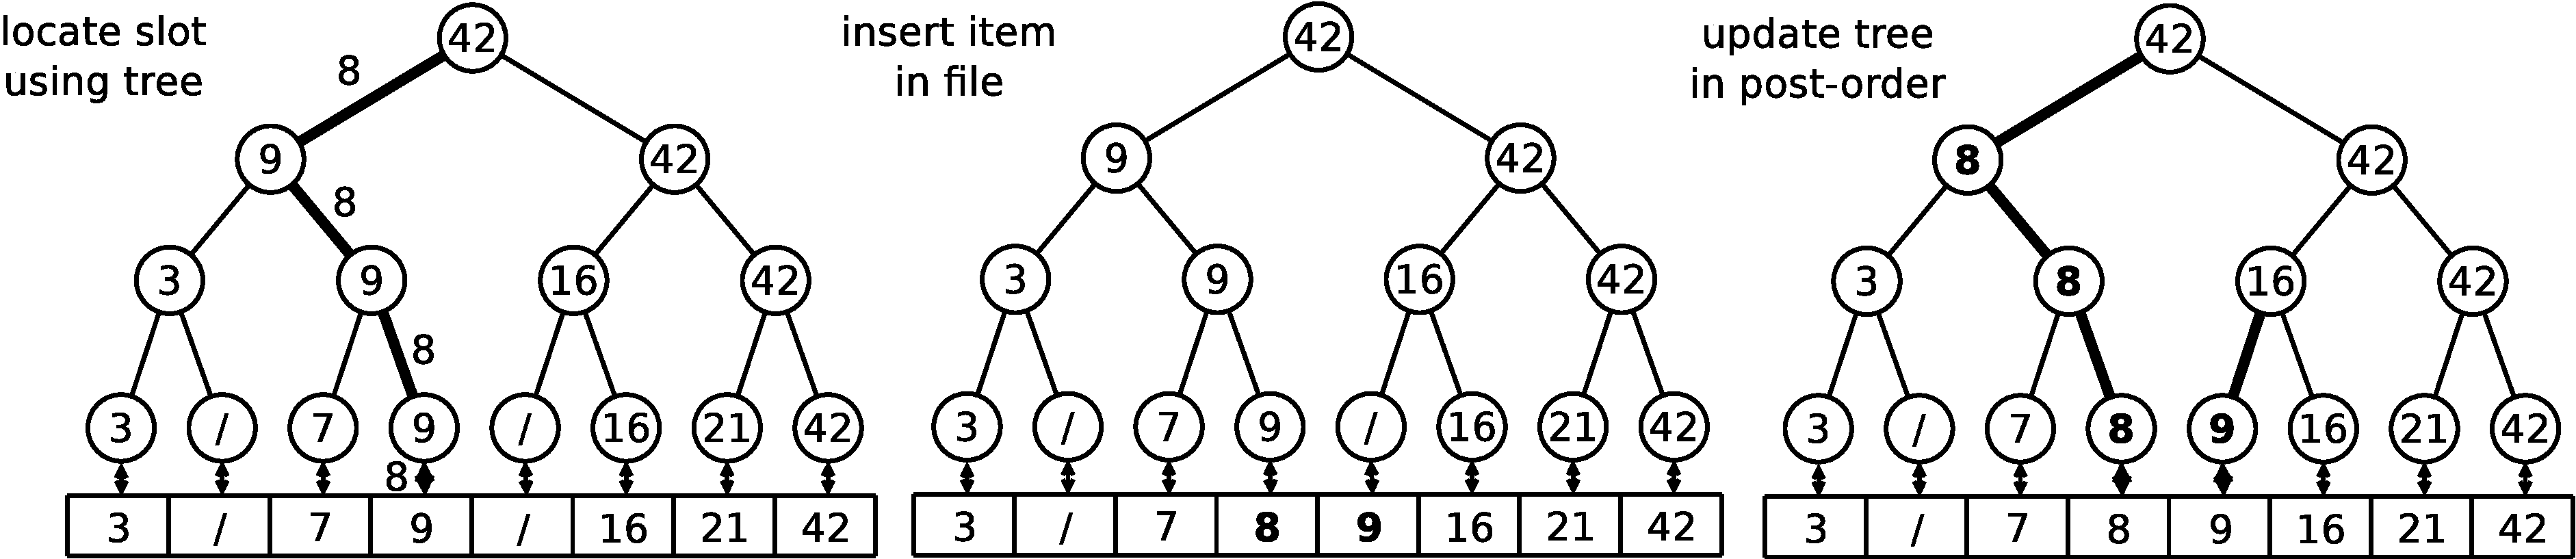
\includegraphics[width=\textwidth]{../figures/downloaded_dont_use/dyn-insert.pdf}
    \end{center}
\end{frame}

\begin{frame}[plain]
\begin{center}
{\Large Ďakujem za pozornosť!}
\vspace{10em}

\url{https://github.com/lacop/thesis} 
\url{https://github.com/lacop/alg-vis}
\end{center}
\end{frame}

\end{document}